\documentclass[10pt]{article}

\usepackage[margin=0.85in]{geometry}
\usepackage[T1]{fontenc}
\usepackage{lmodern}
\usepackage{microtype}
\usepackage{amsmath,amssymb,mathtools}
\usepackage{booktabs}
\usepackage{array}
\usepackage{siunitx}
\usepackage{xcolor}
\usepackage{hyperref}
\usepackage{natbib}
\usepackage{enumitem}
\usepackage{float}
\usepackage{tikz}
\usepackage{pgfplots}
\pgfplotsset{compat=1.18}
\usetikzlibrary{arrows.meta,positioning}
\hypersetup{colorlinks=true,linkcolor=blue!55!black,citecolor=blue!55!black,urlcolor=blue!55!black}
\sisetup{round-mode=places,round-precision=6}
\newcommand{\ddfs}{\textsc{DDFS}}
\newcommand{\mase}{\operatorname{MASE}}
\title{When Drift-Directed Sharing Hurts:\\
A Registered Development-Stage Falsification in Online Load Forecasting}
\author{Anonymous research artifact}
\date{October 21, 2026}

\begin{document}
\maketitle

\begin{abstract}
Online expert aggregation offers a lightweight way to adapt forecasts under
distribution shift, but a plausible drift response need not improve prediction.
We evaluate a causal drift-directed fixed-share policy (\ddfs) that combines three
recursive least-squares experts and changes both the amount and target of shared
probability mass when a common loss detector rises. A preregistered $2\times2$
factorial design isolates adaptive share rate from directed redistribution, while
Hedge, AdaHedge, a uniform ensemble, and seasonal naive provide additional controls.
A private, CPU-only Kaggle run evaluated ten regional electricity-load series for
366 daily forecasts each after a one-year warm-up. The exact 23-file source payload
passed 25 hosted tests, and a separate standard-library verifier recomputed all
metrics from 3,660 retained predictions. Contrary to the hypothesis, \ddfs\ was
worse than constant fixed share by $0.003195$ MASE (synchronized seven-day
moving-block 95\% interval $[0.001469,0.004908]$), with zero favorable series.
Directed redistribution and adaptive sharing were each separately unfavorable;
\ddfs\ was also worse than AdaHedge by $0.010253$ MASE. Both registered advancement
gates therefore failed, and protected confirmation was not opened. The study is a
reproducible development-stage falsification: it identifies a consistent failure of
this transition policy on one correlated load domain, but does not establish
cross-domain generality, a confirmatory null effect, or state of the art.
\end{abstract}

\section{Introduction}

Non-stationary time series tempt forecasters to react whenever recent loss rises.
Fixed-share aggregation provides a principled mechanism for tracking changing
experts \citep{herbster1998tracking}, and forgetting-factor recursive least squares
(RLS) provides a resource-light family of adaptive predictors. Combining the two
suggests an intuitive policy: detect deterioration, increase probability sharing,
and direct that mass toward short-memory experts that currently appear reliable.
Intuition alone, however, is not evidence. Changing the share rate and its target
simultaneously introduces two mechanisms, either of which may increase variance,
overreact to common shocks, or dilute a well-performing expert.

We test this idea under causal prequential evaluation. The proposed policy, \ddfs,
uses the same RLS expert bank and loss sequence as every aggregation control.
A common detector prevents the treatment from changing its own drift trigger. Four
factorial modes distinguish constant versus adaptive share rate and uniform versus
directed share target. AdaHedge \citep{derooij2014follow} supplies a tuning-free
adaptive aggregation comparator.

The contribution is deliberately a falsification study rather than a claimed new
online-learning theory. The real-data development run produced three findings:
\begin{enumerate}[leftmargin=*]
  \item \ddfs\ degraded the registered primary endpoint relative to constant fixed
  share on all ten series, with an uncertainty interval entirely on the harmful side.
  \item Both components were separately unfavorable: adaptive sharing hurt at a
  uniform target, and directed redistribution hurt at a constant share rate.
  \item AdaHedge and ordinary Hedge were the two best registered aggregators, so the
  extra drift machinery did not compensate for its added behavioral complexity.
\end{enumerate}
The protocol required advancement gates before protected confirmation. Because both
failed, stopping is the scientifically valid terminal action.

\section{Related Work}

Fixed share and variable share were introduced for tracking a changing best expert
\citep{herbster1998tracking}; subsequent analysis clarified adaptive-regret
properties and optimality conditions \citep{adamskiy2016closer}. General
time-varying transition matrices over experts fit the MarkovHedge framework
\citep{mourtada2017efficient}, so non-uniform redistribution is not novel by itself.
This work evaluates one particular causal transition heuristic and claims no new
regret bound.

Online aggregation has a substantial electricity-forecasting history.
\citet{devaine2013forecasting} aggregate specialized experts for load prediction,
while adaptive forgetting in RLS has also been studied for this domain
\citep{ba2012adaptive}. AdaHedge adapts the Hedge learning rate through the
mixability gap \citep{derooij2014follow}; Bernstein online aggregation provides
stronger second-order methodology under stated assumptions
\citep{wintenberger2017optimal}. We include AdaHedge but not a BOA implementation,
which rules out broad claims of best online aggregation.

Modern drift-aware time-series systems such as OneNet \citep{zhang2023onenet} and
LEAF \citep{chen2025leaf} use much larger learned architectures and multivariate
benchmarks. They provide field context rather than protocol-matched head-to-head
baselines for this CPU-constrained univariate study. MASE follows
\citet{hyndman2006another}, with its denominator computed only from the warm-up
segment.

\section{Problem Formulation}

For a univariate stream $y_1,\ldots,y_T$, a forecaster emits $\hat y_t$ using only
$y_{<t}$ and observes $y_t$ afterward. Each series has season $s=7$. The
training-only scale is
\begin{equation}
  c_{\mathrm{MASE}} =
  \frac{1}{n-s}\sum_{t=s+1}^{n}\lvert y_t-y_{t-s}\rvert,
\end{equation}
where $n$ is the end of the warm-up period. For method $a$, the series-level
endpoint is
\begin{equation}
  \mase_a = \frac{1}{T-n}\sum_{t=n+1}^{T}
  \frac{\lvert \hat y_{a,t}-y_t\rvert}{c_{\mathrm{MASE}}}.
\end{equation}
Series receive equal weight. The registered primary estimand is
$\Delta=\mase_{\ddfs}-\mase_{\mathrm{fixed}}$; lower is better. Advancement
requires both $\Delta\leq -0.01$ and at least 1\% relative improvement. A mechanism
claim additionally requires favorable \ddfs-minus-adaptive-share performance that
is not reversed in a majority of series.

\section{Method}

\subsection{Shared recursive expert bank}

Expert $i$ uses forgetting factor
$\lambda_i\in\{0.90,0.97,0.995\}$ and an RLS residual model with lags
$\{1,2,3\}$. With seasonal base $b_t=y_{t-s}$ and causal robust scale $c_t$,
\begin{equation}
  \hat y_{i,t}=b_t+c_t\,
  \operatorname{clip}(\hat r_{i,t},-8,8).
\end{equation}
All methods receive identical expert predictions and update the experts only after
the current forecast is recorded. The capped normalized expert loss is
\begin{equation}
  \ell_{i,t}=\min\left(
    \frac{\lvert \hat y_{i,t}-y_t\rvert}{c_t},8
  \right).
\end{equation}

\subsection{Common detector and posterior}

To prevent mode-dependent detector feedback, all modes use the mean expert-bank loss
$d_t=K^{-1}\sum_i\ell_{i,t}$. Fast and slow exponential averages are
\begin{align}
  F_t &= 0.8F_{t-1}+0.2d_t,\\
  S_t &= 0.98S_{t-1}+0.02d_t,
\end{align}
and the drift score is
\begin{equation}
  z_t=\operatorname{clip}\left(
  \frac{F_t-S_t}{\max(S_t,0.05)},0,1\right).
\end{equation}
After observing $y_t$, fixed-rate Hedge forms
\begin{equation}
  q_{i,t+1}=
  \frac{w_{i,t}\exp(-\eta\ell_{i,t})}
       {\sum_jw_{j,t}\exp(-\eta\ell_{j,t})},
  \qquad \eta=0.35.
\end{equation}

\subsection{Rate and target factorial}

The constant rate is $\alpha_0=0.01$; the adaptive rate is
\begin{equation}
  \alpha_t=\operatorname{clip}(\alpha_0+0.02z_t,\alpha_0,0.03).
\end{equation}
The uniform target is $u_i=1/K$. The directed target combines a short-memory
preference $m_i\propto 1-\lambda_i+10^{-3}$ with relative causal expert loss
$p_{i,t}$:
\begin{equation}
  r_{i,t}\propto\sqrt{m_ip_{i,t}},\qquad
  g_{i,t}=(1-z_t)u_i+z_tr_{i,t}.
\end{equation}
The next weights are
\begin{equation}
  w_{i,t+1}=(1-\alpha_t)q_{i,t+1}+\alpha_th_{i,t},
\end{equation}
where the $2\times2$ design selects constant or adaptive $\alpha$ and uniform or
directed $h$. The four cells are fixed share, adaptive share, directed fixed share,
and \ddfs. Figure~\ref{fig:pipeline} summarizes the causal order.

\begin{figure}[t]
\centering
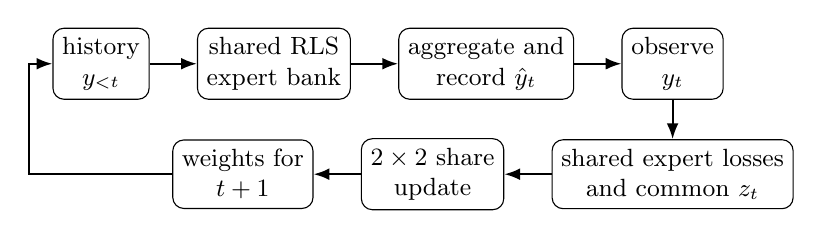
\begin{tikzpicture}[
  node distance=5mm and 6mm,
  box/.style={draw,rounded corners,align=center,minimum height=8mm,font=\small},
  arrow/.style={-{Latex[length=2mm]},thick}
]
\node[box] (history) {history\\$y_{<t}$};
\node[box,right=of history] (experts) {shared RLS\\expert bank};
\node[box,right=of experts] (predict) {aggregate and\\record $\hat y_t$};
\node[box,right=of predict] (observe) {observe\\$y_t$};
\node[box,below=of observe] (loss) {shared expert losses\\and common $z_t$};
\node[box,left=of loss] (update) {$2\times2$ share\\update};
\node[box,left=of update] (next) {weights for\\$t+1$};
\draw[arrow] (history)--(experts);
\draw[arrow] (experts)--(predict);
\draw[arrow] (predict)--(observe);
\draw[arrow] (observe)--(loss);
\draw[arrow] (loss)--(update);
\draw[arrow] (update)--(next);
\draw[arrow] (next.west) -| ([xshift=-3mm]history.west) |- (history.west);
\end{tikzpicture}
\caption{Causal execution order. The current outcome enters only after the current
forecast is recorded. Expert states and detector inputs are shared across factorial
controls.}
\label{fig:pipeline}
\end{figure}

\section{Analytical Properties}

\paragraph{Proposition 1 (control equivalence).}
Suppose all aggregation modes start with identical expert states and observe the
same stream. Then at each time they have identical expert predictions, expert losses,
expert-state updates, and common detector score $z_t$; only aggregation weights and
therefore ensemble forecasts may differ.

\paragraph{Proof.}
At initialization the claim holds by construction. Assume it holds before time $t$.
Each expert prediction is a deterministic function of its own common state and
$y_{<t}$, hence is identical across modes. After $y_t$ is revealed, every mode forms
the same componentwise expert-loss vector. The expert RLS update depends on the
common feature, target, and prior expert state, not on ensemble weights, so the next
expert states agree. The detector is a deterministic function of the mean of this
common loss vector and its shared previous state, so its next score also agrees.
Induction proves the result. \(\square\)

This proposition identifies the implemented controls, not a general causal effect
outside the registered streams. A longitudinal test of the corresponding software
invariant is included in the 25-test hosted suite.

With $K$ experts and RLS feature dimension $d$, each timestamp requires
$O(Kd^2)$ time and $O(Kd^2+W)$ memory, where $W$ is the interval-residual window.
Aggregation itself is $O(K)$. No empirical runtime advantage is claimed because
matched timing and peak-memory measurements were not collected.

\section{Experimental Setup}

\paragraph{Data.}
The registered source is the CC0 Kaggle ``Hourly Energy Consumption'' dataset.
Ten named regional PJM files were aggregated to daily arithmetic means from
2015-01-01 through 2016-12-31. Days with fewer than 20 finite positive hourly
observations are rejected; no interpolation is used. The 365 days of 2015 provide
warm-up and scale estimation; all 366 days of 2016 are evaluated. The loader requires
both boundary dates and daily consecutiveness. Dates from 2017 onward are protected
and were never parsed by this runner.

\paragraph{Methods.}
We evaluate seasonal naive, a uniform RLS ensemble, Hedge, AdaHedge, constant fixed
share, adaptive share, directed fixed share, and \ddfs. The expert bank, features,
outcomes, causal ordering, and evaluation rows are shared. The full configuration is
frozen in the run manifest.

\paragraph{Inference.}
For each contrast, timestamp-level scaled absolute-error differences are resampled
with synchronized moving blocks of seven days across the ten aligned series. This
preserves shared regional shocks. We use 5,000 repetitions and seed 20261021, then
take equal-series means. Development intervals are selection evidence, not
confirmatory inference.

\paragraph{Execution and provenance.}
The private Kaggle version used CPU only, disabled GPU and internet, and ran Python
3.13.15 with NumPy 2.1.3. Before evaluation it checked all 23 source files against
the uploaded manifest and passed 25 tests. The run retained 3,660 raw prediction
rows. Archive and inner-file SHA-256 digests were verified after download. A separate
standard-library script recomputed every reported point metric and contrast without
importing the research package.

\section{Main Results}

\begin{table}[H]
\centering
\caption{Equal-series mean MASE on the registered 2016 development window. Lower is better; every method has 3,660 timestamp-level predictions.}
\label{tab:results}
\begin{tabular}{r l S[table-format=1.6]}
\toprule
Rank & Method & {Mean MASE} \\
\midrule
1 & AdaHedge & 0.614409 \\
2 & Hedge & 0.614465 \\
3 & Fixed share & 0.621467 \\
4 & Directed fixed share & 0.621916 \\
5 & Adaptive share & 0.623639 \\
6 & \textsc{DDFS} & 0.624662 \\
7 & Uniform ensemble & 0.662893 \\
8 & Seasonal naive & 1.026540 \\
\bottomrule
\end{tabular}
\end{table}


Figure~\ref{fig:mase} shows that AdaHedge and Hedge were the strongest registered
aggregators. \ddfs\ did improve substantially over seasonal naive, but this does not
support the hypothesis because simpler matched ensembles improved more.

\begin{figure}[t]
\centering
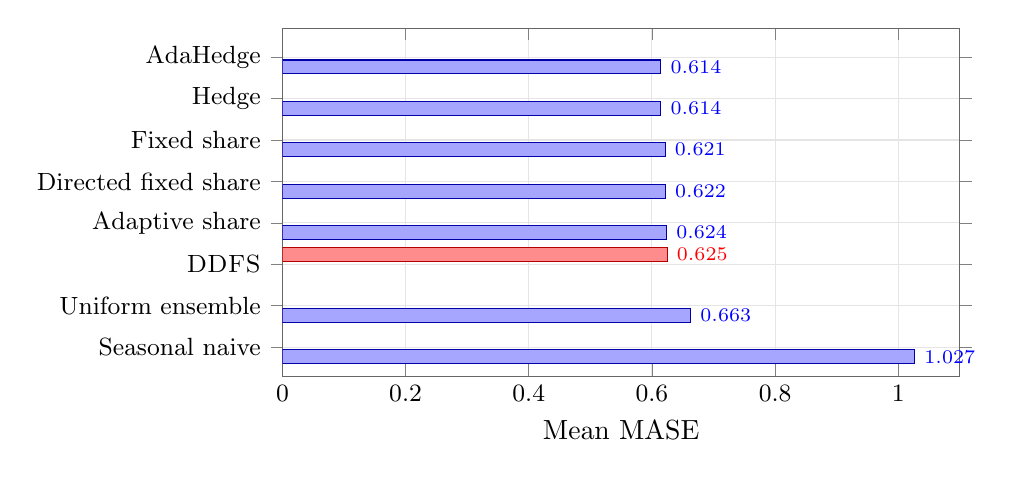
\begin{tikzpicture}
\begin{axis}[
  xbar,
  width=0.84\linewidth,
  height=6.0cm,
  xmin=0,
  xmax=1.10,
  xlabel={Mean MASE},
  ytick={0,1,2,3,4,5,6,7},
  yticklabels={Seasonal naive,Uniform ensemble,\textsc{DDFS},Adaptive share,Directed fixed share,Fixed share,Hedge,AdaHedge},
  yticklabel style={font=\small},
  xticklabel style={font=\small},
  bar width=5pt,
  nodes near coords,
  nodes near coords style={font=\scriptsize,/pgf/number format/fixed,/pgf/number format/precision=3},
  grid=major,
  grid style={gray!20},
  axis line style={black!60},
]
\addplot+[draw=blue!65!black,fill=blue!35] coordinates {(0.614409082,7) (0.614464765,6) (0.621467303,5) (0.621915883,4) (0.623638880,3) (0.662893327,1) (1.026539640,0)};
\addplot+[draw=red!70!black,fill=red!45] coordinates {(0.624662497,2)};
\end{axis}
\end{tikzpicture}

\caption{Equal-series mean MASE; lower is better. Values are regenerated from the
retained analysis JSON. \ddfs\ is highlighted.}
\label{fig:mase}
\end{figure}

The primary \ddfs-minus-fixed-share estimate is positive, indicating harm:
$0.003195$ MASE with 95\% interval $[0.001469,0.004908]$. Its bootstrap probability
of improvement is 0.0 at the retained Monte Carlo resolution, and all ten series
have positive differences. Relative improvement is $-0.5141\%$, so neither the
absolute nor relative advancement criterion is met.

\section{Ablation and Mechanism Analysis}

The factorial controls directly attribute the failure. Adaptive share minus fixed
share is $0.002172$ MASE; directed fixed share minus fixed share is $0.000449$.
Thus each component is harmful in isolation on this domain. Combining them produces
a larger $0.003195$ degradation. \ddfs\ minus adaptive share is $0.001024$, so the
directed target adds harm even when the rate is already adaptive. \ddfs\ minus
directed fixed share is $0.002747$, so rate adaptation adds harm when the target is
already directed. Each of these effects is unfavorable on all ten series.

\begin{figure}[t]
\centering
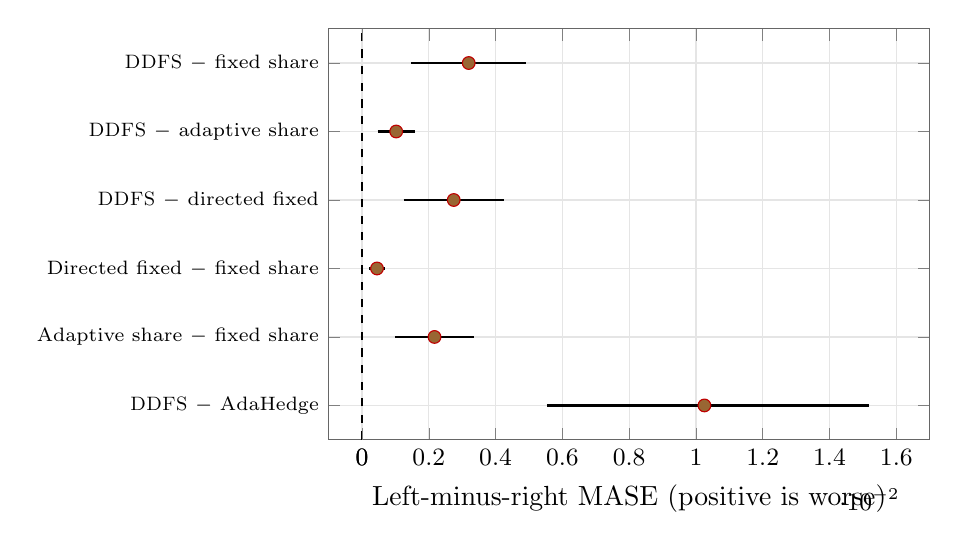
\begin{tikzpicture}
\begin{axis}[
  width=0.76\linewidth,
  height=6.8cm,
  xmin=-0.001,
  xmax=0.017,
  xlabel={Left-minus-right MASE (positive is worse)},
  ytick={0,1,2,3,4,5},
  yticklabels={\textsc{DDFS} $-$ AdaHedge,Adaptive share $-$ fixed share,Directed fixed $-$ fixed share,\textsc{DDFS} $-$ directed fixed,\textsc{DDFS} $-$ adaptive share,\textsc{DDFS} $-$ fixed share},
  yticklabel style={font=\scriptsize},
  xticklabel style={font=\small},
  grid=major,
  grid style={gray!20},
  axis line style={black!60},
  extra x ticks={0},
  extra x tick style={grid=major,grid style={black,dashed,thick}},
]
\addplot[black,thick,mark=none] coordinates {(0.001469058,5) (0.004907738,5)};
\addplot[black,thick,mark=none] coordinates {(0.000466181,4) (0.001580707,4)};
\addplot[black,thick,mark=none] coordinates {(0.001247223,3) (0.004240128,3)};
\addplot[black,thick,mark=none] coordinates {(0.000207960,2) (0.000687862,2)};
\addplot[black,thick,mark=none] coordinates {(0.000980533,1) (0.003360222,1)};
\addplot[black,thick,mark=none] coordinates {(0.005537159,0) (0.015176084,0)};
\addplot+[only marks,mark=*,mark size=2.3pt,red!75!black] coordinates {(0.003195193,5) (0.001023616,4) (0.002746613,3) (0.000448580,2) (0.002171577,1) (0.010253415,0)};
\end{axis}
\end{tikzpicture}

\caption{Registered mean MASE contrasts with synchronized moving-block 95\%
intervals. Positive values favor the right-hand method and therefore contradict the
proposed mechanism.}
\label{fig:contrasts}
\end{figure}

Compared with AdaHedge, \ddfs\ is worse by $0.010253$ MASE, again on all ten series.
This does not establish AdaHedge as universally superior, but it rules out a
competitive-aggregation claim for \ddfs\ under the registered development protocol.

\section{Robustness and Generalization}

The synchronized bootstrap addresses temporal autocorrelation and shared regional
shocks within the evaluated grid. Per-series consistency is unusually clear: every
registered mechanism contrast has zero favorable series. The evidence is nevertheless
limited to correlated load regions from one source and one calendar year. No second
domain, perturbation study, model-scaling experiment, or matched resource benchmark
was executed. Those absences are not silently reclassified as robustness evidence.

The protocol's protected segment was intended only for a candidate that passed
development. Opening it after a uniform adverse result would convert the final test
into another search opportunity. Accordingly, no protected result exists and no
confirmatory null claim is made.

\section{Discussion}

The negative result is mechanistically informative. The base RLS bank is capable:
Hedge and AdaHedge reach mean MASE near 0.614, well below seasonal naive. The failure
therefore does not arise merely because the experts are unusable. Constant fixed
share is worse than Hedge but better than every drift-directed factorial cell.
The registered detector appears to add sharing precisely when concentration on a
successful expert may be valuable; directing mass toward short-memory experts adds
another consistent penalty. Because the experiment was not designed to estimate a
general response function for $z_t$, this interpretation remains a hypothesis rather
than a proven failure law.

A tempting response would be to invert the target, reduce the gain, or select a
different detector after seeing these outcomes. That would be a new, data-informed
hypothesis. It cannot retroactively rescue revision 2 and must receive a separate
identity, protocol, and evaluation budget.

\section{Limitations}

The study has six central limitations. First, it is development-stage evidence and
cannot support a confirmatory population claim. Second, the ten series share one grid
and are not ten independent domains. Third, the expert bank is intentionally small
and linear. Fourth, BOA-class and modern deep online systems were not reproduced
under a matched protocol. Fifth, runtime and peak memory were not measured
comparatively. Sixth, execution and independent metric recomputation were
first-party; no independent researcher has reproduced the package. These limitations
prevent submission-readiness and any SOTA statement.

\section{Conclusion}

A plausible drift-directed fixed-share policy failed a preregistered real-data
development test. \ddfs\ was worse than constant fixed share, adaptive share,
directed fixed share, Hedge, and AdaHedge, with zero favorable series in every key
mechanism contrast. Exact source verification, hosted testing, retained predictions,
synchronized-block uncertainty, and an independent recomputation script make this a
strong negative artifact. The correct scientific conclusion is to reject advancement
of revision 2 and preserve the protected data. Future work, if pursued, must begin as
a separately registered successor rather than tune against or overwrite this result.

\bibliographystyle{plainnat}
\begingroup
\sloppy
\bibliography{references}
\endgroup

\appendix
\section{Complete Configuration}

The registered forgetting factors are $(0.90,0.97,0.995)$; lags are $(1,2,3)$;
ridge is 10; fixed Hedge rate is 0.35; base and maximum shares are 0.01 and 0.03;
drift gain is 0.02; detector rates are 0.20 and 0.02; prediction and loss clips are
both 8; interval level is 90\% with a 256-step residual window.

\section{Complete Registered Contrasts}

\begin{table}[h]
\centering
\small
\caption{All preregistered development contrasts. Positive estimates mean the left-hand method has higher (worse) MASE. Intervals use 5,000 synchronized seven-day moving-block draws.}
\label{tab:contrasts}
\begin{tabular}{l r l r}
\toprule
Contrast & Estimate & 95\% interval & Left wins \\
\midrule
\textsc{DDFS} $-$ fixed share & 0.003195 & [0.001469, 0.004908] & 0/10 \\
\textsc{DDFS} $-$ adaptive share & 0.001024 & [0.000466, 0.001581] & 0/10 \\
\textsc{DDFS} $-$ directed fixed & 0.002747 & [0.001247, 0.004240] & 0/10 \\
Directed fixed $-$ fixed share & 0.000449 & [0.000208, 0.000688] & 0/10 \\
Adaptive share $-$ fixed share & 0.002172 & [0.000981, 0.003360] & 0/10 \\
\textsc{DDFS} $-$ AdaHedge & 0.010253 & [0.005537, 0.015176] & 0/10 \\
\bottomrule
\end{tabular}
\end{table}


\section{Reproducibility and Artifact Identities}

The source archive manifest identity is:
\par\noindent\texttt{4548ba0486279fa45706aa61412ea4efb3bd90803996f38ab708fe7a10a53ebc}.\par
The downloaded result archive identity is:
\par\noindent\texttt{742326e430bc01a15a08151edfe3c198f348e2cbfe0a17e23c1dfa34dc06e4a4}.\par
Inner identities are:
\begin{itemize}[leftmargin=*]
  \item manifest:
  \texttt{a204d446cefc2270}\allowbreak\texttt{e4fd64b1b811063c}\allowbreak
  \texttt{3e087158cbc41370}\allowbreak\texttt{4a66deb07d114af9};
  \item predictions:
  \texttt{31fd1332e8861597}\allowbreak\texttt{e804e3afd125c72a}\allowbreak
  \texttt{fcfded8a1bfc3180}\allowbreak\texttt{c075d21e1dcd1e76};
  \item summary:
  \texttt{844e33655d6d0eff}\allowbreak\texttt{2df608401a8ef91d}\allowbreak
  \texttt{c6711d9d85eeb88e}\allowbreak\texttt{aff2731a8dd4979e}.
\end{itemize}
From the repository root, the independent audit command is:
\begin{verbatim}
.venv/bin/python -S scripts/verify_development_v2.py \
  --artifact-root artifacts/kaggle-development-v2-r1
\end{verbatim}
Paper assets are regenerated from the retained analysis with:
\begin{verbatim}
.venv/bin/python -S scripts/generate_paper_assets.py
\end{verbatim}

\section{Validity Checklist}

No protected date was parsed; the current outcome follows the current prediction;
all factorial cells use identical experts and common detector inputs; all ten
registered files and all 366 evaluation days are present; every method is reported;
negative contrasts are retained; confidence intervals respect temporal and
cross-series dependence; no SOTA, cross-domain, efficiency, or independent-
reproduction claim is made.

\section{Per-Series Primary Effects}

\begin{table}[H]
\centering
\small
\caption{Per-series primary development effects. Positive values indicate higher (worse) MASE for \textsc{DDFS} than constant fixed share.}
\label{tab:series-effects}
\begin{tabular}{l r l}
\toprule
Series & Difference & Direction \\
\midrule
AEP & 0.002987 & Unfavorable \\
COMED & 0.004370 & Unfavorable \\
DAYTON & 0.004299 & Unfavorable \\
DEOK & 0.001996 & Unfavorable \\
DOM & 0.003405 & Unfavorable \\
DUQ & 0.002961 & Unfavorable \\
EKPC & 0.002911 & Unfavorable \\
FE & 0.003625 & Unfavorable \\
PJME & 0.002801 & Unfavorable \\
PJMW & 0.002596 & Unfavorable \\
\bottomrule
\end{tabular}
\end{table}


\end{document}
